\documentclass{minimal}
\usepackage{graphicx,color}
\usepackage[utf8]{inputenc}
\usepackage[papersize={418.00bp,314.00bp},text={418.00bp,314.00bp}]{geometry}
\begin{document}
\centering
% Title: gl2ps_renderer figure
% Creator: GL2PS 1.4.2, (C) 1999-2020 C. Geuzaine
% For: Octave
% CreationDate: Mon Dec 12 16:45:05 2022
\setlength{\unitlength}{1pt}
\begin{picture}(0,0)
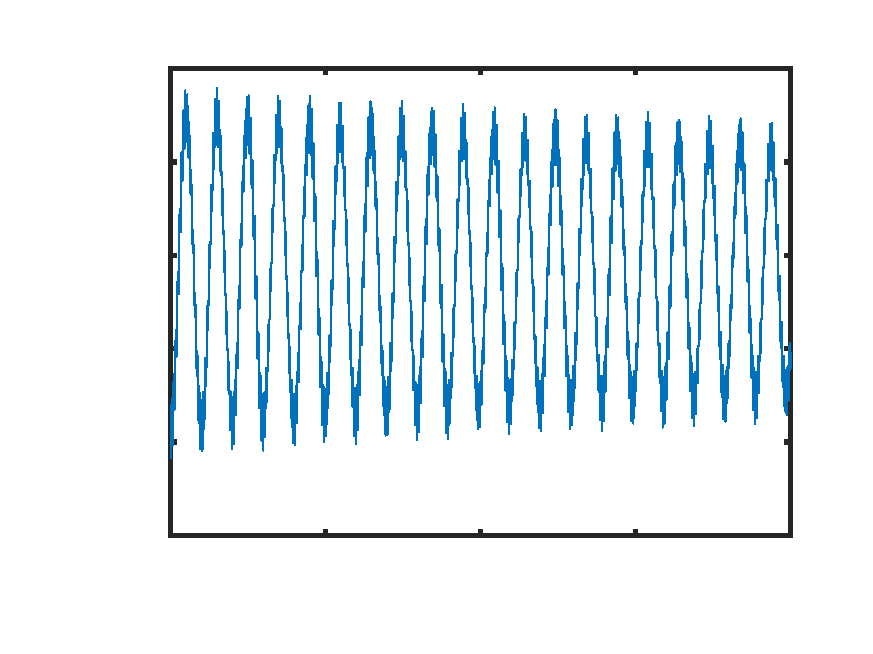
\includegraphics[scale=1]{DoubleKapitzaTimeSeriesTheta1-inc}
\end{picture}%
\begin{picture}(418,314)(0,0)
\fontsize{22}{0}\selectfont\put(81.9981,40.9559){\makebox(0,0)[t]{\textcolor[rgb]{0.15,0.15,0.15}{{0}}}}
\fontsize{22}{0}\selectfont\put(141.388,40.9559){\makebox(0,0)[t]{\textcolor[rgb]{0.15,0.15,0.15}{{20}}}}
\fontsize{22}{0}\selectfont\put(200.777,40.9559){\makebox(0,0)[t]{\textcolor[rgb]{0.15,0.15,0.15}{{40}}}}
\fontsize{22}{0}\selectfont\put(260.167,40.9559){\makebox(0,0)[t]{\textcolor[rgb]{0.15,0.15,0.15}{{60}}}}
\fontsize{22}{0}\selectfont\put(319.557,40.9559){\makebox(0,0)[t]{\textcolor[rgb]{0.15,0.15,0.15}{{80}}}}
\fontsize{22}{0}\selectfont\put(378.946,40.9559){\makebox(0,0)[t]{\textcolor[rgb]{0.15,0.15,0.15}{{100}}}}
\fontsize{22}{0}\selectfont\put(71,57.4247){\makebox(0,0)[r]{\textcolor[rgb]{0.15,0.15,0.15}{{3}}}}
\fontsize{22}{0}\selectfont\put(71,102.14){\makebox(0,0)[r]{\textcolor[rgb]{0.15,0.15,0.15}{{3.05}}}}
\fontsize{22}{0}\selectfont\put(71,146.855){\makebox(0,0)[r]{\textcolor[rgb]{0.15,0.15,0.15}{{3.1}}}}
\fontsize{22}{0}\selectfont\put(71,191.57){\makebox(0,0)[r]{\textcolor[rgb]{0.15,0.15,0.15}{{3.15}}}}
\fontsize{22}{0}\selectfont\put(71,236.285){\makebox(0,0)[r]{\textcolor[rgb]{0.15,0.15,0.15}{{3.2}}}}
\fontsize{22}{0}\selectfont\put(71,281){\makebox(0,0)[r]{\textcolor[rgb]{0.15,0.15,0.15}{{3.25}}}}
\fontsize{24}{0}\selectfont\put(230.472,18.9559){\makebox(0,0)[t]{\textcolor[rgb]{0.15,0.15,0.15}{{Time}}}}
\fontsize{24}{0}\selectfont\put(24,169.212){\rotatebox{90}{\makebox(0,0)[b]{\textcolor[rgb]{0.15,0.15,0.15}{{$\theta_1$}}}}}
\fontsize{24}{0}\selectfont\put(230.472,291){\makebox(0,0)[b]{\textcolor[rgb]{0,0,0}{{Time Series of $\theta_1$}}}}
\end{picture}
\end{document}
